% Sección B · Arquitectura y operación de la cadena (componente B, 25 %). Reemplaza a la «Cadena ejecutable» de la E1.
% Requiere en el preámbulo: graphicx, booktabs, array, xcolor. Las cifras salen de E2/output/cifras.md y dq_resultados.csv.
\providecommand{\pend}[1]{\textcolor{red}{#1}}

\section{Arquitectura y operación de la cadena}
\label{sec:arquitectura}

La cadena de la E1 corría en un computador. Ahora corre en Databricks Free Edition como un job de ocho pasos, con las tablas en Unity Catalog, pruebas de calidad antes de publicar y un tablero que lee el resultado (figura~\ref{fig:arquitectura}).

\paragraph{Cómo se corre de cero.} En un workspace de Free Edition se crea una carpeta Git con el repositorio (\emph{Workspace $\rightarrow$ Create $\rightarrow$ Git folder}) y se ejecuta \emph{Run all} en \texttt{E2/correr\_e2}. Ese notebook crea el job \texttt{vallehondo\_e2}, lo ejecuta, muestra las pruebas y las cifras y publica el tablero, sin instalar nada ni configurar credenciales: las fuentes van en el repositorio. Demora unos 6 minutos. Sobre un catálogo vacío reprodujo byte a byte el registro de limpieza de la E1. El 17 de noviembre la corrimos en un workspace nuevo, de otra cuenta, siguiendo solo el README: 8 de 8 pasos terminaron bien, pasaron las 15 pruebas y salieron las mismas cifras del informe. Tardó unos 14 minutos, 6 de ellos esperando el primer cómputo de la cuenta nueva; la API del dólar no respondió y la cadena usó el respaldo. La ventana para crear la carpeta Git quedó cargando, así que la creamos con la misma URL desde la API; el README lo explica.

\begin{figure}[!htbp]
  \centering
  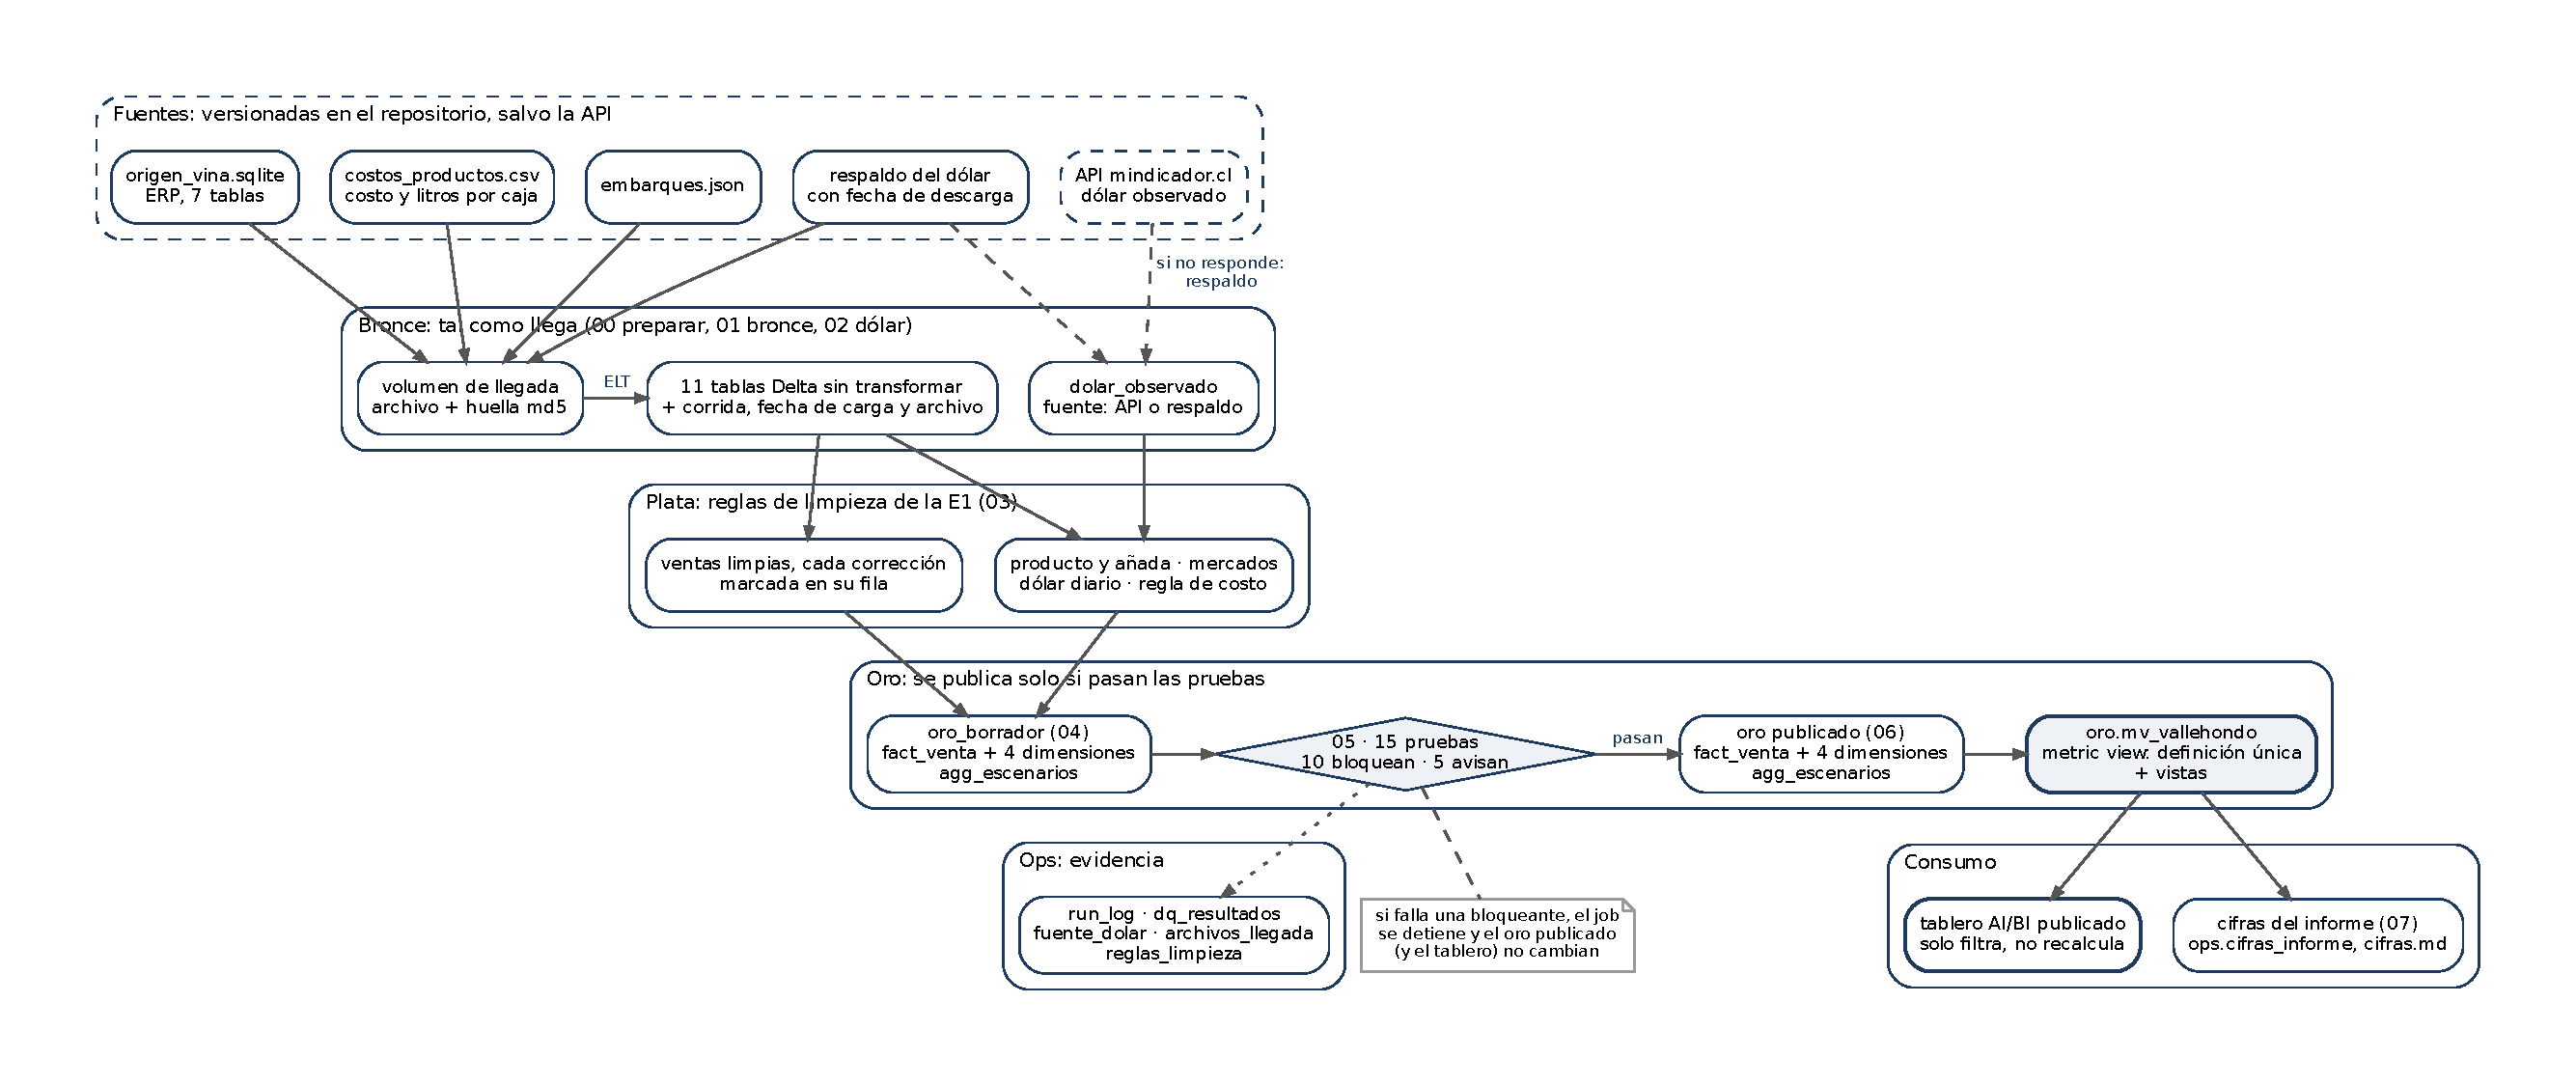
\includegraphics[width=0.82\textwidth]{arquitectura.pdf}
  \caption{Arquitectura por capas. Los números entre paréntesis son los pasos del job. Fuente: elaboración propia.}
  \label{fig:arquitectura}
\end{figure}

\paragraph{Qué hace cada capa.} \textbf{Bronce} guarda las cuatro fuentes tal como llegan, como tablas Delta, con la corrida, la fecha de carga y el archivo de origen. \textbf{Plata} aplica las reglas de limpieza de la E1 (anexo~B); cada corrección queda marcada en su fila, y eso permite apagarla. \textbf{Oro} tiene el modelo de la sección~\ref{sec:modelo}, la tabla de escenarios y la definición única de la métrica; se arma en un esquema borrador y se publica solo si las pruebas lo permiten. \textbf{Ops} guarda la evidencia de cada corrida: pasos, pruebas y origen del dólar. El \textbf{tablero} solo filtra; no recalcula nada.

\paragraph{Tres decisiones.}
\begin{itemize}\setlength\itemsep{1pt}
\item \textbf{ELT y no ETL.} Las fuentes entran crudas a bronce y se transforman dentro de Databricks. Si cambia una regla, como los litros por caja, se reprocesa desde bronce sin volver a extraer, y el linaje queda en una sola plataforma. El costo: depender de la cuota diaria de cómputo de Free Edition.
\item \textbf{Carga completa en cada corrida.} Todas las tablas se reemplazan, nunca se agregan: con 13.845 líneas la corrida dura minutos, y agregar sobre lo anterior duplicaría ventas si un paso se reintenta. Una prueba compara cada corrida con el oro publicado: dos corridas dejan 13.845 líneas y USD 73.435.428,61.
\item \textbf{Si la API del dólar falla, respaldo con fecha; si no hay respaldo, no se publica.} Desde Databricks, mindicador.cl responde a veces: en la corrida oficial respondió para 2025 y no para 2026 (M). Cuando falla, la cadena usa el respaldo versionado en el repositorio (descargado el 2 y el 12 de octubre de 2026), lo registra, y el pie del tablero muestra la fuente y su fecha. Si ninguno cubre una fecha, la prueba del dólar bloquea y el tablero sigue mostrando la última corrida buena.
\end{itemize}

\paragraph{Pruebas de calidad.} Quince pruebas corren en cada ejecución, entre el oro borrador y su publicación. Diez \emph{bloquean} el job si fallan: una por fuente (ERP, JSON, CSV y dólar) y las que protegen la métrica (clave única del hecho, sin huérfanos, fechas dentro del período, conciliación entre plata y oro). Cinco \emph{avisan}: rangos de precio y descuento, cifras de control de la E1, idempotencia y los dos pisos del acuerdo de servicio. El anexo~B detalla qué verifica cada una, qué hace si falla y su resultado en la última corrida.

\paragraph{Linaje.} Unity Catalog dibuja solo el linaje entre tablas. La figura~\ref{fig:linaje} lo completa hasta la pantalla para cada campo de la métrica: de qué columna sale, qué regla lo corrige, en qué campo del hecho queda y dónde se ve. El ingreso, por ejemplo, nace en el precio, el descuento, el monto y la moneda de la venta; pasa por los 555 montos recalculados y las 542 monedas imputadas; queda en \texttt{monto\_neto\_usd} y llega al tablero como numerador de \texttt{precio\_por\_litro}.

\begin{figure}[!htbp]
  \centering
  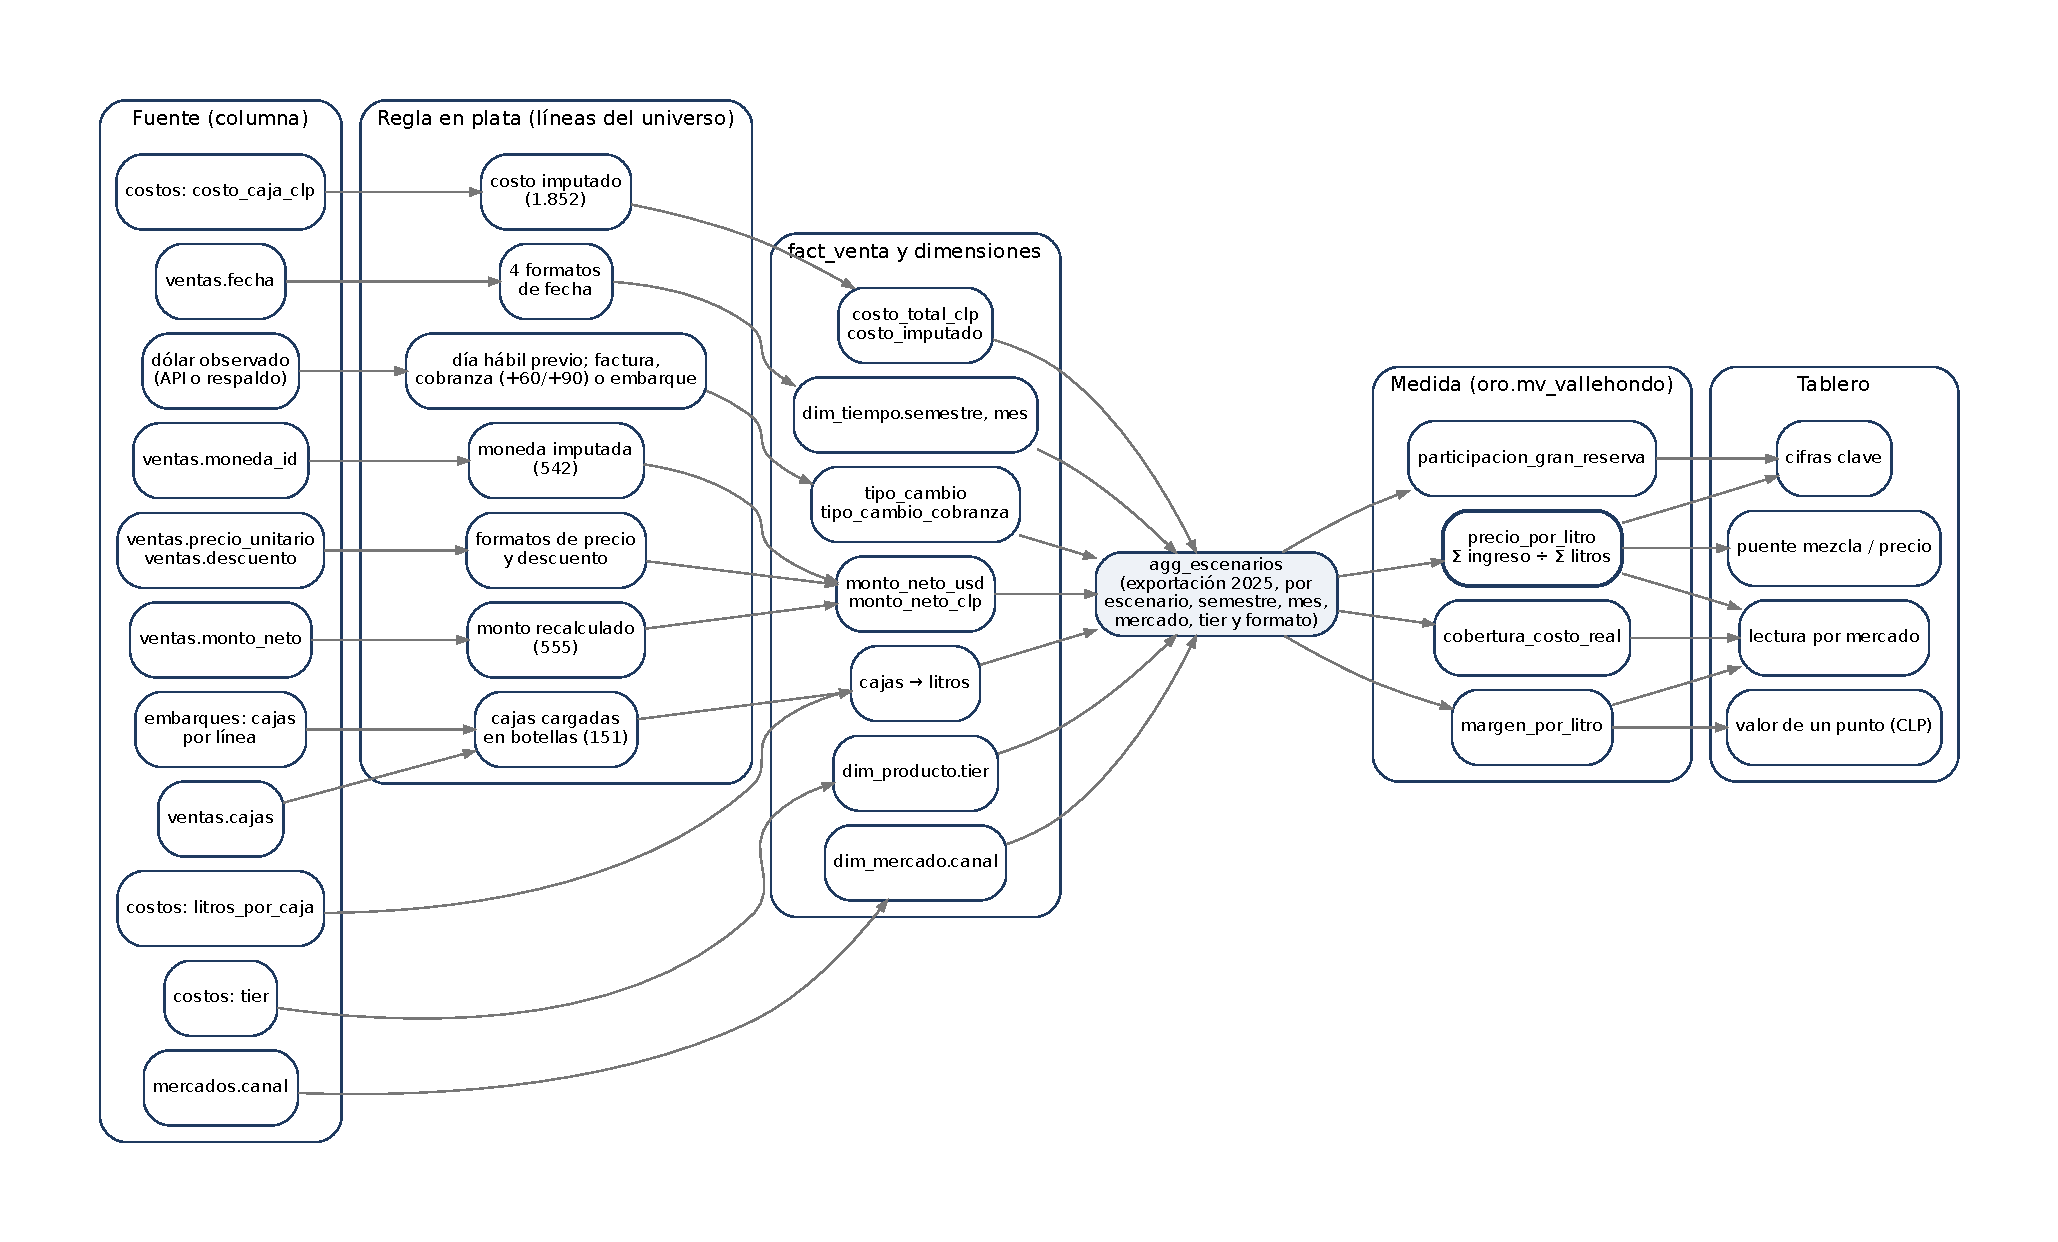
\includegraphics[width=0.56\textwidth]{linaje.pdf}
  \caption{Linaje de la métrica, de la columna de origen a la pantalla. Fuente: elaboración propia a partir del código de la cadena.}
  \label{fig:linaje}
\end{figure}

\paragraph{Acuerdo de servicio de \texttt{fact\_venta}.} Los dos pisos de completitud se miden en cada corrida como pruebas que avisan, y la frescura con la fecha de la última corrida; el pie del tablero muestra las tres cosas.

\begin{center}\footnotesize
\renewcommand{\arraystretch}{1.15}
\begin{tabular}{@{}l p{5.6cm} p{6.4cm}@{}}
\toprule
\textbf{Compromiso} & \textbf{Valor} & \textbf{Por qué ese umbral} \\
\midrule
Frescura & Mensual, a más tardar 5 días hábiles después del cierre & Comercial arma hoy la cifra una vez al mes (V) \\
Completitud & Al menos 98\,\% de las ventas registradas llega a \texttt{fact\_venta}; al menos 80\,\% de los litros con costo real & Hoy llegan 99,0\,\% y hay 82,8\,\% con costo real; bajo esos pisos el margen deja de ser defendible (M) \\
Calidad & 100\,\% de las pruebas que bloquean y al menos 90\,\% del total en verde & Una prueba que bloquea en rojo es un número que no se puede defender \\
Dueño & Departamento Comercial & Es quien hoy descarga el ERP y arma la cifra mensual (V) \\
\bottomrule
\end{tabular}
\end{center}

